\section{Datasets}
\label{sec:datasets}

This section briefly discusses and analyzes the datasets used in our experiments.


\subsection*{GovReport}

Introduced by \citet{huang-etal-2021-efficient}, this dataset consists of reports written by government research agencies, including the Congressional Research Service (CRS) and the U.S. Government Accountability Office (GAO).
Exact word count information is given in \autoref{tab:datasets}.
\autoref{fig:govreport} shows the word count distribution of the dataset.

\begin{figure}[!ht]
  \centering
  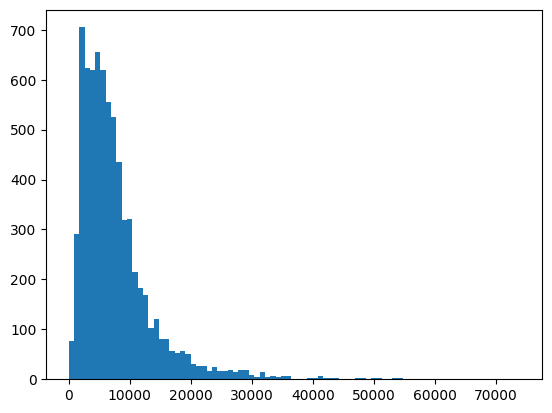
\includegraphics[width=.48\textwidth]{images/govreport-wordcount.png}
  \caption{
    Histogram of GovReport word counts.
    The x-axis represents document word counts, while the y-axis shows the number of documents.
  }
  \label{fig:govreport}
\end{figure}


\subsection*{BigPatent}

Introduced by \citet{sharma-etal-2019-bigpatent}, this dataset consists of over 1.3 million records of U.S. patent documents with human-written abstractive summaries.
Exact word count information is given in \autoref{tab:datasets}.
\autoref{fig:bigpatent} shows the word count distribution of the dataset.

\begin{figure}[!ht]
  \centering
  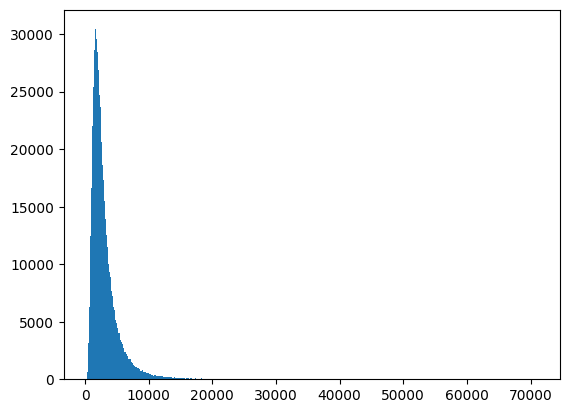
\includegraphics[width=.48\textwidth]{images/bigpatent-wordcount.png}
  \caption{
    Histogram of BigPatent word counts.
    The x-axis represents document word counts, while the y-axis shows the number of documents.
  }
  \label{fig:bigpatent}
\end{figure}


\begin{table*}[!ht]
  \centering

  \begin{tabular}{c c c c}
    \hline
    Dataset & Avg. Word Count & Max Word Count & No. of Documents \\
    \hline
    GovReport & 7,700.71 & \textbf{73,815} & 7,238 \\
    BigPatent & 3,055.72 & \textbf{71,027} & 1,341,362 \\
    \hline
  \end{tabular}

  \caption{Dataset information}
  \label{tab:datasets}
\end{table*}
